\documentclass[11pt,titlepage]{article}
\usepackage[reqno]{amsmath}
\usepackage{amssymb}
\usepackage{epsf}
\usepackage{epsfig}
\usepackage{url}

% === additional commands/packages/settings ===
\usepackage{graphicx,psfrag,natbib}
\usepackage{setspace}
\usepackage{vmargin}
\setpapersize{USletter}

% === dcolumn package ===
\usepackage{dcolumn}
\newcolumntype{.}{D{.}{.}{-1}}
\newcolumntype{d}[1]{D{.}{.}{#1}}

% === newcommands from sei.tex ===
\newcommand{\EI}{\ensuremath{{\mathfrak EI}}}
\newcommand{\Tiny}{\tiny}
\newcommand{\sump}{\sum_{i=1}^p}
\newcommand{\mean}{\frac{1}{p}\sump}
\newcommand{\ub}{\Dot{\beta}}
\newcommand{\ut}{\Dot{\theta}}
\newcommand{\bbeta}{{\mathfrak B}}
\newcommand{\btheta}{{\mathfrak T}}
\newcommand{\blambda}{{\mathfrak L}}
\newcommand{\bbetau}{\breve{\mathfrak B}}
\newcommand{\bV}{{\cal V}}
\newcommand{\sigmau}{\breve{\sigma}}
\newcommand{\Sigmau}{\breve{\Sigma}}
\newcommand{\rhou}{\breve{\rho}}
\newcommand{\psiu}{\breve{\psi}}
\newcommand{\Eu}{\breve{\text{E}}}
\newcommand{\Vu}{\breve{\text{V}}}
\newcommand{\Bb}{B^b}
\newcommand{\Bw}{B^w}
\newcommand{\NbD}{{N_i^{bD}}}
\newcommand{\NwD}{{N_i^{wD}}}
\newcommand{\NbR}{{N_i^{bR}}}
\newcommand{\NwR}{{N_i^{wR}}}
\newcommand{\NbN}{{N_i^{bN}}}
\newcommand{\NwN}{{N_i^{wN}}}
\newcommand{\tp}{{\mbox{\Tiny{+}}}}
\newcommand{\NpD}{{N_i^D}}
\newcommand{\NpR}{{N_i^{R}}}
\newcommand{\NpN}{{N_i^{N}}}
\newcommand{\Nbp}{{N_i^{b}}}
\newcommand{\Nwp}{{N_i^{w}}}
\newcommand{\Npp}{{N_i}}
\newcommand{\Nppp}{{N}}
\newcommand{\Nbpp}{{N^{b}}}
\newcommand{\Nwpp}{{N^{w}}}
\newcommand{\sumpN}{\sump\Npp}
\newcommand{\NsumpN}{\frac{1}{\Nppp}\sumpN}
\newcommand{\nbp}{{N_i^{bT}}}
\newcommand{\nwp}{{N_i^{wT}}}
\newcommand{\npp}{{N_i^{T}}}
\newcommand{\NbV}{{N_i^{bT}}}
\newcommand{\NwV}{{N_i^{wT}}}
\newcommand{\NpV}{{N_i^{T}}}
\newcommand{\xb}{\bar{X}}
\newcommand{\wb}{\bar{W}}
\newcommand{\tb}{\bar{T}}
\newcommand{\cx}{{\mathbb X}}
\newcommand{\cw}{{\mathbb W}}
\newcommand{\ct}{{\mathbb T}}
\newcommand{\cpij}{{\mathbb P}^*_{ij}}
\newcommand{\cpi}{{\mathbb P}^*_i}
\newcommand{\cwd}{{\dot{\mathbb W}}}
\newcommand{\ctd}{{\dot{\mathbb T}}}
\newcommand{\cxd}{{\dot{\mathbb X}}}
\newcommand{\cxb}{\bar{\mathbb X}}
\newcommand{\cz}{{\mathbb G}}
\newcommand{\ch}{{\mathbb H}}
\newcommand{\cm}{{\mathbb M}}
\newcommand{\E}{{\textbf{E}}}
\newcommand{\V}{{\textbf{V}}}
\newcommand{\C}{{\textbf{C}}}
\newcommand{\rE}{{\text{E}}}
\newcommand{\rV}{{\text{V}}}
\newcommand{\rC}{{\text{C}}}
\newcommand{\TN}{\text{TN}}
\newcommand{\BN}{\text{BN}}
\newcommand{\N}{\text{N}}
\renewcommand{\P}{\text{P}}
\newcommand{\D}{\textbf{D}}
\newcommand{\R}{\ensuremath{\textbf{R}}}
\newcommand{\Rr}{\ensuremath{\{\textbf{R}\diagdown r}\}}
\newcommand{\bC}{\ensuremath{\textbf{C}}}
\newcommand{\Cc}{\ensuremath{\{\textbf{C}\diagdown c}\}}
\newcommand{\one}{{\mathbf{1}}}
\newcommand{\Q}{\ensuremath{\overset{\vspace{3em}}{\text{\Huge ?}}}}
\newlength{\padsp}
\settowidth{\padsp}{$(\beta^w_i=\nwp/\Nwp)$}
\newcommand{\padbw}{\hspace*\padsp}
\newcommand{\bkappa}{\boldsymbol{\kappa}}

\newcommand{\bb}{\beta^{\text{bad}}}
\newcommand{\bg}{\beta^{\text{good}}}
\renewcommand{\bibitem}{\vskip 2pt\par\hangindent\parindent\hskip-\parindent}

\title{Analyzing Second-Stage Ecological Regressions\thanks{Our thanks
    to Michael Herron and Kenneth Shotts for helpful comments on an
    earlier draft.}}

\author{Christopher Adolph\thanks{Department of Government, Harvard
    University. (Littauer Center, North Yard, Harvard University,
    Cambridge MA 02138; \texttt{http://chris.adolph.name},
    \texttt{cadolph@fas.harvard.edu}).}
\and %
Gary King\thanks{Department of Government, Harvard University and
  World Health Organization (Center for Basic Research in the Social
  Sciences, 34 Kirkland Street, Harvard University, Cambridge MA
  02138; \texttt{http://GKing.Harvard.Edu}, \texttt{King@Harvard.Edu},
  (617) 495-2027).}  }

\begin{document}
\maketitle

\section{Introduction}

We take this opportunity to comment on Herron and Shotts (2002;
hereinafter HS) because of its interesting and productive ideas and
because of the potential to affect the way a considerable body of
practical research is conducted.  This article, and the literature
referenced therein, is based on the suggestions in three paragraphs in
King (1997: 289--90).  Since these paragraphs were not summarized in
HS, we thought they might be a useful place to start:
\begin{quotation}
  If a second stage analysis is conducted, least squares regression
  should probably not be used in most cases, even though it may not be
  particularly misleading.  The best first approach is usually to
  display a scatterplot of the explanatory variable (or variables)
  horizontally and (say) an estimate of $\beta_i^b$ or $\beta_i^w$
  vertically.  In many cases, this plot will be sufficient evidence to
  complete the second stage analysis.
  
  If it proves useful to have more of a formal statistical approach,
  and many of the actual values of $\beta_i^b$ fall near zero or one,
  then some method should be used that takes this into account.  The
  data could be transformed, via a logit or probit transformation, or
  [the ``extended model''] could be applied\ldots.  Whatever method is
  chosen, the researcher should be careful to include the fact that
  some estimates of $\beta_i^b$ are more uncertain than others.
    
  In practice, a weighted least squares linear regression may be
  sufficient in many applications, with weights based on the standard
  error of $\beta_i^b$ (or other quantity of interest).  Researchers
  should be careful in applying this simplified method here, and
  should verify its assumptions with scatterplots. \ldots This is not
  as theoretically elegant a procedure as the more formal set up in
  [the ``extended model''] but it is simple, relatively robust, and
  probably complete enough to be of use in many applications.
\end{quotation}  

Clearly the only logically consistent model that has been offered for
the issue at hand is the EI extended model that allows the second
stage covariates to be included in the EI estimation procedure.  EI
software now includes a feature that allows for first differences to
be computed if those covariates are included, which should make the
extended model somewhat easier to understand and use.  (We discuss how
to use the extended model in Section \ref{s:exten}.)

Any second stage analysis is by definition a second best
procedure, when judged conditional on the model.  Still, second
stage analyses --- if they give approximately correct answers --- have
the advantage of being easier to understand, use, and evaluate (since
an estimate of the dependent variable in the second stage is
observable), more numerically stable (hence allowing more covariates
to be included and studied), computationally faster (allowing more
analyses to be examined), more amenable to diagnostics in verifying
assumptions (since the actual estimated data points can be observed
and the fit can be checked directly), and possibly more robust to
certain types of misspecification.  The question at hand is if and
when such a procedure can be used to produce answers that are
approximately correct.

HS's contribution is in pointing out that precinct-level estimates
from EI regress to the mean.  This ``shrinkage'' property is indeed a
characteristic of EI, and it is also a characteristic of every other
Bayesian model.  Shrinkage results in optimal estimates, that is, with
the smallest possible mean square error.  Thus, we agree with the
implication of HS's article that the best possible estimate of
$\beta_i^b$ (e.g., the fraction of blacks who vote), under HS's
assumptions, is that produced by EI.  But HS also make the interesting
and correct point that using Bayesian mean posterior estimates with
this property, like those given by EI, as dependent variables in least
squares regression can, under some circumstances, produce biased
estimates.  No one disputes that second stage regressions are
approximations or that they cause problems from some theoretical
perspectives; the question at hand is when they cause problems that
affect real applied research.

HS study second stage regression based on least squares and conclude
that their bias-adjusted slope is preferable.  The article does not
mention whether the constant term should be adjusted.  Their slope
adjustment is based on linear approximations within the classical
linear econometric theory framework.  The problems with HS's approach
we discuss here are due to assuming linearity when modeling an
inherently nonlinear and bounded relationship (i.e., their algebra by
definition miss the information in the bounds), omitting the constant
correction from the paper, never computing the correction they propose
when conducting simulations, and missing the fact that weighted least
squares corrects problems they raise.  We show how filling in this
missing information leads back to the suggestions from the paragraphs
quoted above.

In addition to making second-stage analyses possible by providing the
first precinct-level estimates from an ecological inference model, the
primary advance of EI was in resolving the half-century long debate
between supporters of Goodman's (1959) unbounded linear regression
approach and Duncan-Davis' (1953) method of bounds by incorporating
all information in both into the same model.  HS fall back to
Goodman's unbounded approach and so miss the highly informative
deterministic information in the aggregate data.

We replicated HS's simulations without trouble.  We then examined how
well their adjusted regression procedure fit the observed data based
on the estimated $\hat\beta_i^b$ and the true (normally unobserved)
$\beta_i^b$.  We find that correcting the slope but not the constant
is considerably worse than an unadjusted regression of $\hat\beta_i^b$
on $Z_i$ and the other procedures discussed in HS's paper and the
literature we have examined.  This is true even if we knew the true
value of the adjustment.  Unless $Z$ has zero mean, the regression
line from this method tends to miss the cloud of true $\beta_i^b$
points by a wide margin.

We therefore begin by extending HS's partial adjustment procedure,
within their linear econometric framework, by developing an adjustment
for the constant term.  We follow the procedure that we believe Herron
and Shots would have used if they had done so.\footnote{Indeed, after
  we finished a draft, Herron and Shotts told us that they had the
  same constant correction in a draft version of their paper but took
  it out in the final version to save space.  Since HS suggest
  correcting the slope, and do not mention constant term corrections,
  when we refer to the ``HS partially adjusted procedure,'' we are
  referring to what readers would conclude that Herron and Shotts
  advocate, even though we now know (from our subsequent
  correspondence with them) that they also believe the corrections
  discussed in their paper are incomplete in real applications.}  As
it turns out, this fully adjusted second stage regression method
dominates the slope-only procedure and indeed the partially adjusted
procedure in HS is never called for.

Since the only estimators HS offer for their partial adjustment
procedure either assume knowledge of the truth being estimated or
assume that some unknown parameters can be estimated without error, we
develop an estimator without these flaws and apply it to create full
adjustments.  We find that this fully empirical version of the full
adjustment procedure is, with two partial exceptions, dominated by
(unadjusted) weighted least squares.  For one, when the bounds are
wide, the true adjustment factor could make a noticable difference,
but the adjustment itself cannot be reliably estimated and so the
procedure cannot be applied.  But in this case, of course, researchers
should not be running EI in the first place because of extreme model
dependence.  For the other, nonlinear relationships obviously cannot
be well modeled by any linear second stage regression, and so in that
case a logistic (or other nonlinear) regression procedure is best.
Thus, the only situation when the adjustment would lead to
improvements is when the bounds are wide and the true value of the
adjustment is known, which describes the Monte Carlo procedures HS
used to evaluate their method, but of course not any real application.
(Even in this unrealistic situation, the full correction takes an hour
to run, compared to a few seconds for weighted least squares.)  Since
researchers can easily detect which situation applies from the
available aggregate data, they can always take appropriate action.

We conclude that researchers with narrow enough bounds to run first
stage EI should first examine a scatterplot of the covariate
horizontally by the bounds on $\beta_i^b$ vertically (such as King,
1997: Fig.13.2, p.238), since it requires no assumptions at all, and a
scatterplot of the covariate horizontally by the estimate
$\hat\beta_i^b$ vertically, to check for nonlinearities (which
normally occur when the estimated points are near zero or one).  If
nonlinearities are not apparent, then weighted least squares should be
used since it offers approximately unbiased estimates in second stage
regressions.

\section{A Fully Adjusted Second Stage Regression Model}
\label{s:fulladj}

We try to stick to HS's notation where possible and present the fully
adjusted method with their adjustment as a special case.\footnote{Our
  notation deviates from HS only to ensure logical consistency.  For
  example, their Equations (7) and (8) have different dependent
  variables, $\beta_i^b$ and $\hat\beta_i^b$ set equal to the same
  entire right side of the equation in both cases
  ($\alpha+\gamma'Z_i+\nu_i$).  Later in their paper, they allow
  $\gamma$ to differ between the two (calling the first $\gamma_R$ and
  the second $\gamma_U$), but do not fix the constant term (or error
  terms).  We fix these issues and others, since what they probably
  intended seems clear.}

First, let the expectation of $\beta_i^b$ conditional on $Z_i$ be
approximated by
\begin{equation}
  \label{true}
  E(\beta_i^b)=\alpha_R+\gamma_R Z_i,
\end{equation}
so that estimates of $\alpha_R$ and $\gamma_R$ are the immediate goal
of the analysis.  Also let the expectation of $\hat\beta_i^b$
conditional on $Z_i$ be
\begin{equation}
  \label{est}
  E(\hat\beta_i^b)=\alpha_U+\gamma_U Z_i,
\end{equation}
which is of course well estimated by least squares.  HS then assumes
that the error in estimating $\hat\beta_i^b$ by EI is a linear
function of $\beta_i^b$:
\begin{equation}
  \label{hserr}
  E(\hat\beta_i^b - \beta_i^b) = \delta_0^b + \delta_1^b\beta_i^b.
\end{equation}
Then solving (\ref{hserr}) for $E(\hat\beta_i^b)$ and substituting the
result into (\ref{est}) gives a more informative version of (\ref{true}):
\begin{equation}
  \label{adj}
  E(\beta_i^b) = \left(\frac{\alpha_U-\delta_0^b}{1+\delta_1^b}\right)
  + \left(\frac{\gamma_U}{1+\delta_1^b}\right)Z_i.
\end{equation}
Thus, we know that the quantities of interest, $\alpha_R$ and
$\gamma_R$, can be expressed as the intercept and slope of
(\ref{adj}).  If we can estimate the components of each, we can derive
a consistent estimator, at least when HS's linearity and unboundedness
assumptions are not too far off.

\section{An Improved Estimation Procedure}

HS offer an estimation algorithm for correcting the slope term in
their Section 7.2.  This procedure is intuitive and we can easily
generalize it to provide a correction for the intercept as well.
Unfortunately, the procedure itself is flawed for two other reasons.
First, it conditions on the point estimate for the parameters of the
truncated bivariate normal, $\breve\psi$, and of $\delta$, and thus
assumes the absence of estimation uncertainty.  Ignoring uncertainty
would bias standard errors and confidence intervals, of course, which
perhaps is why HS do not calculate these.  However, since their
estimation procedure is nonlinear (due to the ratios in (\ref{adj})),
ignoring estimation uncertainty also affects their point estimates in
finite samples.  And second, the procedure calls for drawing only a
single simulation of $(\beta_i^b,\beta_i^w)$ for each observation.  As
a result, the estimate includes substantial Monte Carlo approximation
error.  The error can be eliminated by running their entire procedure
many times and averaging.  Although fixing these problems would not
have substantially changed the estimates presented in their paper,
they will matter in some applications.  We therefore develop and use a
new estimation algorithm that corrects these problems, as well as
providing the ability to compute standard errors and confidence
intervals, which were not available in HS's version.\footnote{To
  define our revised estimation algorithm, let a symbol with a tilde
  on it denote a value of that quantity randomly drawn from its
  posterior density.  For a given $X$ and $T$: (1) run EI on $X$ and
  $T$; (2) regress $\hat\beta_i^b$ (which comes from EI) on $Z_i$
  yielding the estimated intercept $\hat\alpha_U$ and slope
  $\hat\gamma_U$; (3) draw $\tilde\psiu$ from its posterior provided
  by EI; (4) take $p$ draws of $(\tilde\beta_i^b,\tilde\beta_i^w)$
  from a truncated normal density with parameter vector $\tilde\psiu$,
  (5) compute a new $T_i$ as $\tilde
  T_i=\tilde\beta_i^bX_i+\tilde\beta_i^w(1-X_i)$; (6) run EI on $X_i$
  and $\tilde T_i$ to yield estimates
  ($\hat{\tilde\beta}_i^b,\hat{\tilde\beta}_i^w$) for all $i$; (7)
  regress ($\hat{\tilde\beta}_i^b-\beta_i^b$) on $\beta_i^b$ to
  estimate $\delta_0^b$ and $\delta_1^b$, which we label
  $\hat{\tilde\delta}_0$ and $\hat{\tilde\delta}_1$; (8) draw
  $\tilde\alpha_U$ and $\tilde\gamma_U$ from the posterior provided by
  LS; (9) compute the adjusted intercept as
  $(\tilde\alpha_U-\hat{\tilde\delta}_0^b)/(1+\hat{\tilde\delta}_1^b)$
  and adjusted slope as $\tilde\gamma_U/(1+\hat{\tilde\delta}_1^b)$;
  (10) repeat steps (3)-(9) a sufficient number of times to eliminate
  Monte Carlo approximation error; (11) and average the simulations in
  (10) to get point estimates, take their standard deviation for
  standard errors, or sort them and use percentile values for
  confidence intervals.}

The accurate procedure which fully represents the uncertainty of HS's
corrections is computationally slow (taking about an hour to do one
run).  Also, the standard errors for the fully adjusted method appear
larger than those obtained from LS by about 70\% and WLS by about
30\%.  For the intercepts, which under full adjustment combine the
uncertainty of three parameters, the standard errors are on average 34
times larger than LS, and 25 times larger than WLS.  Thus, any
reduction in bias that may occur is probably outweighed by the
substantial increase in variance.  This is an intuitive result given
that the bias adjustment takes the form of a ratio, and both the
numerator (which is LS) and denominator contain estimation
uncertainty.  (We confirmed this result with a small number of Monte
Carlo experiments.)  It is also consistent with the experience of
others trying to create bias adjustments in a variety of models
outside the field of ecological inference.

\section{HS's Monte Carlo Simulation Procedure}

We explain in this section that HS's Monte Carlo procedure is
inappropriate for evaluating second stage regressions.  The procedure
is to draw the true value of the dependent variable, $\beta_i^b$, from
the EI model without covariates.  Then they create the covariate for
the second stage explanatory variable $Z_i$ endogenously as equal to
$\beta_i^b$ plus random noise.  This procedure has three serious
flaws.

The first flaw is that the Monte Carlo procedure can be interpreted in
three logicially inconsistent ways.  HS do not discuss which
interpretation they intended, but none of the three are appropriate.
The first, and in our view most plausible, interpretation is that by
creating $Z_i$ with random error, the procedure induces immense
errors-in-variables attenuation bias, quite apart from any attenuation
bias that may occur due to the Bayesian shrinkage in the EI estimate.

This problem can be seen clearly by studying the parameters of the
model HS created from which to draw their Monte Carlo data.  In this
model, the slope of the coefficient on the covariate in the second
stage regression is 1 (in their notation,
$\gamma_R=1$).\footnote{Under the HS Monte Carlo setup,
  $E(\beta_i^b)=\alpha_R+\gamma_R Z_i$, where $Z_i=\beta_i^b+\tau_i$
  and $E(\tau_i)=0$ and so $E(Z_i|\beta_i^b)=\beta_i^b$.  Hence
  $E(\beta_i^b)=\alpha_R+\gamma_RE(\beta_i^b+\tau_i) =
  \alpha_R+\gamma_R\beta_i^b$.  which implies that $\alpha_R=0$ and
  $\gamma_R=1$.}  However, the estimates of this slope from their
simulations of the \emph{true} $\beta_i^b$ (i.e., without any
attenuation bias in the dependent variable at all) regressed on $Z$
gives a drastically biased estimate.  This slope estimate does not
appear in their article, but we were able to to replicate their Table
2 exactly, and in our Table \ref{t:hsrep} present these numbers.  As
can be seen, whereas the theoretical value of $\gamma_R$ is 1 in each
case, their estimates indicate that $\hat\gamma_R\approx 0.07$.  Thus,
since the unadjusted method is unable to recover the coefficients
without shrinkage when using the true value of the dependent variable,
this Monte Carlo setup is inappropriate for assessing a dependent
variable that is estimated (by EI or otherwise).
\begin{table}[tb]
\label{t:hsrep}
\begin{center}
\begin{tabular}{c|cc}
Model Parameters & Truth & \multicolumn{1}{c}{HS Estimates} \\
$\breve\psi$  & $\gamma_R$ & $\hat\gamma_R$ \\\hline
(0.5, 0.5, 0.1, 0.1, 0)  &1      &       0.04\\  
(0.75, 0.5, 0.1, 0.1, 0) &1      &       0.04  \\
(0.75, 0.75, 0.1, 0.1, 0)&1      &       0.04  \\
(0.9, 0.9, 0.1, 0.1, 0)  &1      &       0.02  \\
(0.5, 0.5, 0.32, 0.1, 0) &1      &       0.19  \\
(0.6, 0.6, 0.1, 0.32, 0) &1      &       0.04  \\
(0.9, 0.1, 0.32, 0.32, 0)&1      &       0.15  \\
(0.5, 0.5, 0.1, 0.1, 0.3)&1      &       0.04  \\
\hline
\end{tabular}
\end{center}
\caption{Comparing the true slope on $Z$ in a 
second-stage regression in the HS Monte Carlo 
procedure with the estimate based on $\beta_i^b$ 
(rather than $\hat\beta_i^b$) as the dependent variable.
This table replicates the results of simulations presented in
HS's Table 2.  All results are averages over 100 simulations.  
The difference and ratios presented in HS Table 2 were  
successfully replicated, and are not shown here.}
\end{table}

The Monte Carlo procedure can also be interpreted in two other ways,
neither of which alters the conclusion that it is inappropriate for
the purpose of evaluating second-stage regressions.\footnote{A second
  interpretation of the HS Monte Carlo procedure is that $\gamma_R$ is
  the causal effect of $Z_i$ on $\beta_i^b$.  In fact, since many
  second stage regressions are intended to be causal, this is the most
  appropriate intepretation in some situations.  Since $Z_i$ was
  created endogenously, no matter how one exogenously changes $Z_i$,
  $\beta_i^b$ will not budge, and hence, by this interpretation, the
  Monte Carlo procedure is setting the causal effect to zero:
  $\gamma_R=0$.  Thus, because the rightmost column of Table
  \ref{t:hsrep} is uniformly greater than zero, we know that
  regressing the true $\beta_i^b$ on $Z_i$ overestimates $\gamma_R$.
  Thus, since the unadjusted method is unable to recover the true
  coefficients when using the true value of the dependent variable
  (i.e., even though no shrinkage occurs or estimation error in the
  dependent variable exists), the Monte Carlo setup under this second
  interpretation also is inappropriate for assessing a dependent
  variable that is estimated (by EI or otherwise).
  
  A third way to interpret the true value in HS's simulations is
  conditional on \emph{each} randomly generated set of $\eta_i$'s
  ($i=1,\dots,n$), and hence conditional on each randomly generated
  $Z_i$: $E(\beta_i^b|Z_i)=\alpha_R+\gamma_R Z_i$.  By this
  interpretation, each random draw of a set of $n$ observations from
  the Monte Carlo data generating process produces a \emph{different}
  true value of $\gamma_R$, the value of which is neither set nor
  observed by the researcher.  This value can be estimated by a LS
  regression of the the true $\beta_i^b$ on $Z_i$, and it can also be
  estimated by EI-R.  Even if we assume that the LS estimator is
  better (because it uses the true $\beta_i^b$), comparing the two
  estimators does not reveal which is closer to the unknown
  $\gamma_R$.  Since they are probably correlated, the Monte Carlo
  procedure can only reveal how close the estimators are to each
  other, not to the truth, since it is unknown.  By this
  interpretation, the procedure misses the whole point of running
  Monte Carlo experiments in the first place --- creating a world
  where we know the true quantity being estimated and then seeing how
  good an estimator is at recovering its known value.  Although by
  this interpretation we cannot know the true $\gamma_R$ in each
  iteration, we can compute the expected value by averaging over the
  variability in $\tau_i$ over Monte Carlo iterations, but this then
  implies that on average $\gamma_R=1$, and leads exactly to the first
  interpretation and to a regression of $\beta_i^b$ on $Z_i$
  underestimating the truth.  (That is,
  $E_\eta[E(\beta_i^b|Z_i)]=\alpha_R+\gamma_R \beta_i$ which implies
  that $\alpha_R=0$ and $\gamma_R=1$.)}

Whichever interpretation one has of the HS Monte Carlo procedure, it
also suffers from two other serious problems.  First, it artificially
rules out the possibility of nonlinear relationships between
$\beta_i^b$ and $Z_i$ created by the bounds.  That is, by constructing
the explanatory variable, $Z_i$, from the bounded $\beta_i^b$'s (plus
a normal disturbance), the procedure artificially restricts the
relationship between the two to be linear and to never be affected by
the [0,1] bounds on $\beta_i^b$.  Within this framework, testing the
robustness of the HS adjustment to the sort of nonlinear relationships
which crop up sometimes in applied research is impossible.

Finally, \emph{HS's Monte Carlo simulations do not test the actual
  adjustment procedure they propose}.  All the results they present in
their Section 6 rely on the \emph{true} $\beta_i^b$'s to estimate
$\delta_0^b$ and $\delta_1^b$, even though this is the one quantity
users of second-stage regressions by definition lack.  Appropriately,
HS recommend a different estimation procedure (in their Section 7.2)
for use when $\beta_i^b$ is unknown, but leave this procedure
untested.  Hence, HS's article offers no direct evidence that
adjustment would be less biased or more efficient than unadjusted
least squares in practice.


\section{An Improved Monte Carlo Simulation} \label{s:alt}

Most of our conclusions below do not depend on changing the simulation
method, but we do so in order to make the results more coherent.  To
simulate, we follow the logic of the extended EI model.  Thus, we
first fix $X$, the covariates $Z$ (to values uncorrelated with $X$),
the values for the intercept and the slope parameter on $Z$, and the
variance and covariance parameters of the truncated bivariate normal.
Then, for each simulation, we draw the $\beta_i^b$'s from the extended
EI model conditional on $X_i$ and $Z_i$ (without mean centering).  The
assumption that $X_i$ and $Z_i$ are uncorrelated enables us to run a
(first-stage) basic EI model (i.e., with no covariates) without
inducing aggregation bias.  (The assumption is of course less
important when the bounds are more informative, but we retain it for
simplicity in the simulations below.)  With this setup, unless the
relationship is clearly nonlinear, a regression of the true
$\beta_i^b$ on $Z_i$ recovers the intercept and slope coefficients
accurately, effectively correcting the problem with the HS's
procedure.

We use this Monte Carlo setup to illustrate four prototypical
situations that in our experience map out the space of applications in
which the various second-stage methods work in different ways, at
least when we follow the parameter values chosen in HS.  (That is, all
the simulations we have run look like these plots or, roughly
speaking, convex combinations of them.)

First, when ecological data have very wide bounds, EI (and any method
of ecological inference) will be sensitive to modeling assumptions.
In many applications with data like these, no ecological inference
should be conducted unless one has some special auxiliary information
about the model assumptions.  If one nevertheless proceeds to the
second stage, then, since shrinkage probably exists in the
$\beta_i^b$'s, the true (unobserved) value of the full adjustment
would make for an improvement over least squares using the estimated
$\hat\beta_i^b$'s.  Of course, the true adjustment is not known and
needs to be estimated.  Unfortunately, it cannot be estimated
reliably.  The reason is that EI models $\beta_i^b$ as a random effect
constrained to be within the precinct-level bounds. If $Z_i$ is not in
the EI first stage (which is true by definition, since if it were
included we wouldn't need a second stage), then \emph{the only
  information in $\hat\beta_i^b$ that could be predicted by $Z_i$
  comes from the bounds}.  The same is true of the adjustment
procedure: \emph{the only information with which to estimate
  $\delta_0^b$ and $\delta_1^b$ comes from the bounds}.  If the bounds
are relatively uninformative, as we are assuming in this first
prototypical case, then there is little information with which to
estimate the adjustment.  Of course, this should not be a surprise: an
unbounded random effect variable must be unrelated to all measured
variables except by chance.

Figure \ref{f:wide} plots the covariate $Z_i$ horizontally by the true
$\beta_i^b$ (in the left graph) and the estimated $\hat\beta_i^b$ (in
the right graph) vertically.  Note how the unadjusted least squares
line (marked LS) fits the estimated points well (in the right graph)
but are attenuated for the true points (in the left).  Since the
bounds are all very wide, the variances are almost constant and so the
weighted least squares (marked WLS) line is practically on top of the
LS line.  The line representing the fully adjusted method using the
\emph{true} values of $\delta_0^b$ and $\delta_1^b$ (true adjustment
is marked TA) fits the true points well, and would correct for the
attenuation.  The actual fully adjusted method (marked FA) as
estimated from the data also appears, but due to the wide bounds it is
not a good estimate and indeed is worse than LS and WLS.  Figure
\ref{f:wide} also plots the partially adjusted method that a
researcher might implement based on HS's article (marked PA), which is
more biased than any of the alternatives, a problem which grows in
severity as the mean of $Z$ departs from zero (The HS and FA lines are
not exactly parallel because HS is calculated by assuming the estimate
$\hat\psiu$ is known exactly whereas FA uses our estimation
procedure.)  Since the partially adjusted method is never better than
full adjustment, and often dramatically worse, we do not consider it
further.
\begin{figure}[t]
  \begin{center}
    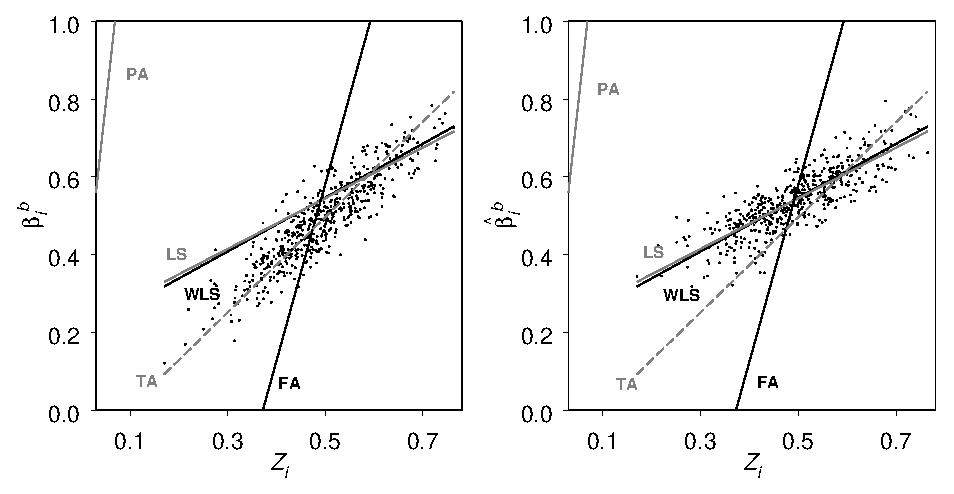
\epsfig{file=wide.eps, width=5.5in}
    \caption{Data with Wide Bounds. Plot of $Z_i$ horizontally by
      the estimated $\hat\beta_i^b$ vertically (in the right graph)
      and the true $\beta_i^b$ (in the left graph), with fits for the
      partially adjusted procedure (PA) in HS, least squares (LS) and
      weighted least squares (WLS) almost on top of one another, the
      fully adjusted method (FA), and the full adjustment based on the
      true values of $\delta_0^b$ and $\delta_1^b$ (TA).  Clearly TA
      fits the true points best, but is unfortunately badly estimated
      by FA.  In this example, insufficient information exists in the
      bounds with which to make ecological inferences at all.  Data
      were generated from the extended EI model with $X \sim
      \textrm{Uniform}(0,0.2)$, $Z \sim \textrm{Normal}(0.5,0.01)$,
      $\breve\bbeta_i^b = Z_i - 0.1$, $\breve\bbeta_i^w = Z_i - 0.1$,
      $\sigmau_b = 0.05$, $\sigmau_w = 0.05$, and $\rhou = 0$.}
    \label{f:wide}
  \end{center}
\end{figure}

Second, when the bounds are at least somewhat informative (that is,
when few of the bounds are extremely wide), we are in the situation
when we would be more likely to trust ecological inferences using EI
(or another method that takes into account the information in the
precinct-level bounds).  When in addition the relationship is
approximately (or locally) linear, we find that least squares and
weighted least squares usually do as well as, and often better than,
the fully adjusted procedure.  Figure \ref{f:narrow} gives one example
where least squares, weighted least squares, and the fully adjusted
method all give approximately the same estimates.
\begin{figure}[t]
  \begin{center}
    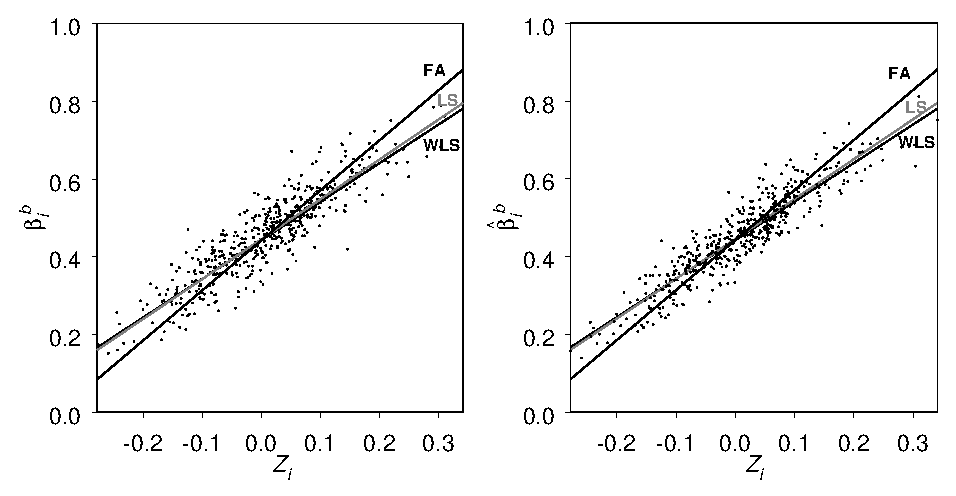
\epsfig{file=narrow.eps, width=5.5in}
    \caption{Data with Informative Bounds. Plot of the $Z_i$ horizontally by
      the estimated $\hat\beta_i^b$ vertically (in the right graph)
      and the true $\beta_i^b$ (in the left graph) with fits for least
      squares (LS) and weighted least squares (WLS) appears almost on
      top of one another, and the fully adjusted method (FA).  Note
      how all three methods give almost the same answer. Data were
      generated from the extended EI model, with $X \sim
      \textrm{Uniform}(0.2,1)$, $Z \sim \textrm{Normal}(0,0.01)$,
      $\breve\bbeta_i^b = Z_i + 0.44$, $\breve\bbeta_i^w = Z_i +
      0.68$, $\sigmau_b = 0.05$, $\sigmau_w = 0.05$, and $\rhou = 0$.}
    \label{f:narrow}
  \end{center}
\end{figure}

Third, when some observations have wide bounds and others have narrow
bounds, and $\hat\beta_i^b$ is an approximate (or locally) linear
function of $Z_i$, (unadjusted) weighted least squares regression will
often be substantially less biased than least squares, and
approximately equivalent to or better than the fully adjusted
procedure.\footnote{Like all weighted regressions, this procedure
  would have higher variance than LS. HS studied consistency, and
  implicitly bias, but did not address other properties, such as
  efficiency.}  This is contrary to
HS's claims that WLS would not make a difference; what they missed by
applying a linear regression framework to this problem with bounds and
nonlinearity is that the degree of attenuation is greater when the
bounds are wider --- as can be seen by the differences between Figures
\ref{f:wide} and \ref{f:narrow} --- and so the weights are correlated
with the attenuation bias and can at least partially correct for it.

Figure \ref{f:mixed} provides an example of this phenomenon.  We
generated the data for this figure from the same model as Figure
\ref{f:narrow}, changing only the parameter values so that the points
were affected by the bounds.  The effect of the wide bounds on some
observations can be seen by the attenuation in the set of points
forming a flatter slope in the right graph (as compared to the left
graph which has no such feature).  As a result, the least squares (LS)
line is a good deal flatter than it should be (as judged by the fit to
the points in the left graph) but the (unadjusted) weighted least
squares (WLS) line corrects for most of the attenuation.  The fully
adjusted (FA) line, in contrast, over-corrects for attenuation.
\begin{figure}[t]
  \begin{center}
    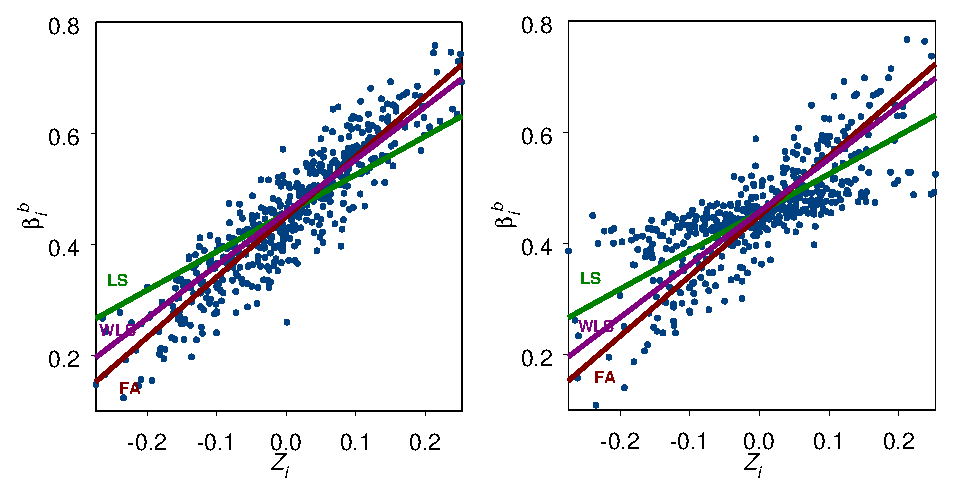
\epsfig{file=mixed.eps, width=5.5in}
    \caption{Data with Narrow and Wide Bounds. Plot of the $Z_i$ 
      horizontally by the estimated $\hat\beta_i^b$ vertically (in the
      right graph) and the true $\beta_i^b$ (in the left graph) with
      fits for least squares (LS), weighted least squares (WLS), and
      the fully adjusted method (FA).  Note how (unadjusted) WLS
      corrects for most of the attenuation bias.  Data were generated
      from the extended EI model, with $X \sim
      \frac{1}{2}\textrm{Uniform}(0,0.2) +
      \frac{1}{2}\textrm{Uniform}(0.8,1)$, $Z \sim
      \textrm{Normal}(0,0.01)$, $\breve\bbeta_i^b = Z_i + 0.44$,
      $\breve\bbeta_i^w = Z_i + 0.68$, $\sigmau_b = 0.05$, $\sigmau_w
      = 0.05$, and $\rhou = 0$.}
    \label{f:mixed}
  \end{center}
\end{figure}

Finally, when the relationship is nonlinear, as is often observably
the case because of the bounds, then any (adjusted or unadjusted)
linear second stage procedure can produce impossible results.  In this
situation, a scatterplot or an appropriate nonlinear procedure would
be better.  The fully adjusted procedure in this situation often
produces more out of bounds predictions than the unadjusted procedure.
(In this case, WLS is also inappropriate, both because the assumption
of linearity does not hold, and because $\hat\beta_i^b$'s at the
extremes have standard errors of zero or nearly so.  Giving extra
weight to these observations tends to bias the estimate of the slope
downwards.)  Figure \ref{f:nonlinear} illustrates these issues.  In
this example, we also include a nonlinear model by using a loess
regression of a logit transformation of $\hat\beta_i^b$,
$\ln(\hat\beta_i^b/(1-\hat\beta_i^b))$, on $Z_i$ and using simulation
to compute the regression line.  This line (marked loess) clearly
gives a far better fit than any of the other methods.  It is also the
only method that does not extend above 1 or below 0 for $\beta_i^b$
(i.e., into the impossible region) for some values of $Z_i$.  (A
linear regression on the logit scale would also stay out of the
impossible region but the fit would not be as much of an improvement.)
\begin{figure}[t]
  \begin{center}
    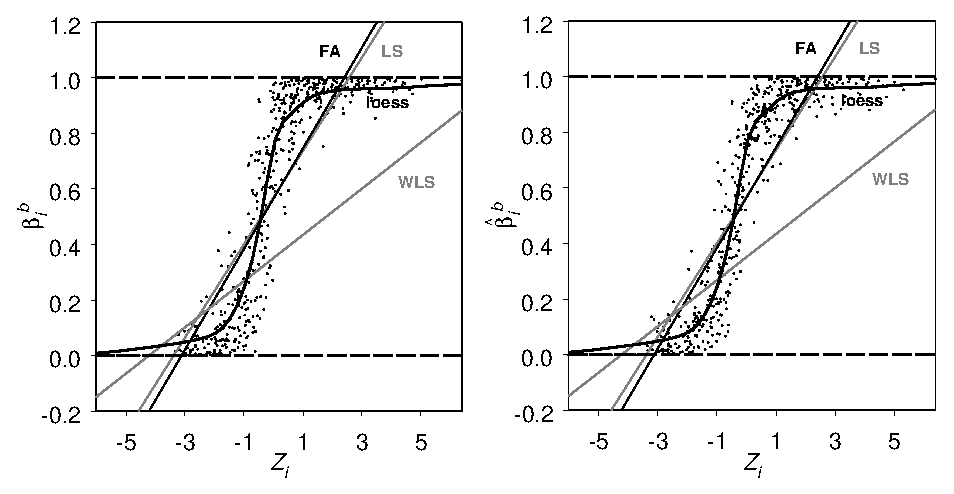
\epsfig{file=nonlinear.eps, width=5.5in}
    \caption{Data with a Nonlinear Relationship.  Plot of $Z_i$ 
      horizontally by the estimated $\hat\beta_i^b$ vertically (in the
      right graph) and the true $\beta_i^b$ (in the left graph) with
      fits for least squares (LS) and the fully adjusted method (FA)
      almost on top of one another, weighted least squares (WLS), and
      the better fitting loess regression on the logistic scale
      (loess).  Note how all the linear methods give out of bounds
      predictions.  Data were generated from the extended EI model,
      with $X \sim \textrm{Uniform}(0,1)$, $Z \sim
      \textrm{Normal}(0,4)$, $\breve\bbeta_i^b = Z_i + 1.16$,
      $\breve\bbeta_i^w = Z_i + 1.16$, $\sigmau_b = 0.3$, $\sigmau_w =
      0.3$, and $\rhou = 0$.}
    \label{f:nonlinear}
  \end{center}
\end{figure}

\section{The Extended Model} \label{s:exten}

As the only self-consistent ``second-stage'' approach, the extended
model should probably see more use.  We therefore pause briefly here
to discuss an important issue about how to use it.  

One apparently obvious, but flawed, way to use the extended model is
to study the effects of the explantory variables only by looking at
the parameter estimates ($\alpha^b$ and $\alpha^w$ in King, 1997: 170)
and their standard errors.  The problem with this approach is that it
does not include the robustness of the bounds that comes from
conditioning on $T$.  

To explain, consider a simpler case: estimating the district-wide
fraction of blacks who vote, $B^b$ without covariates.  If the model
holds (and the number of people per precinct is constant over
precincts), a consistent and efficient estimator of this quantity is
as follows.  (1) Run EI to estimate the five parameters of the
truncated bivariate normal.  Since they are on the untruncated scale,
(2) compute from them (analytically or by simulation) the truncated
parameters, which of course includes the mean of the precinct
parameters and hence our estimate.

Suppose, however, that the model is not exactly right.  Then we would
also want to condition on $T$ so that the precinct-level bounding
information can be included in this estimate.  To do this, use an
alternative estimator: (1) Run EI to estimate the five parameters of
the truncated bivariate normal.  Then (2) condition on $T$ and compute
estimates of the fraction of blacks who vote in each precinct,
$\beta_i^b$, by drawing (as in King, 1997) from the posterior density,
$\P(\beta_i^b|T_i)$, all the mass of which falls within the known
bounds.  Finally, (3) average the precinct estimates to produce an
estimate of $B^b$, as desired originally.

Because it includes the precinct-level bounds, the second estimator is
clearly more robust to misspecification than the first.  And since
dealing with misspecification is the key issue in making ecological
inferences in real research, we see little reason to use the first
estimator.  An equivalent problem applies in estimating and
interpreting $\alpha^b$ and $\alpha^w$ directly: the estimates do not
include information from the precinct-level bounds.  Although
conditional on the model, they are consistent and efficient, they will
not be as robust to misspecification.  Thus, we suggest the same
robust approach to estimating effects from the extended model: (1)
Estimate the parameters of the truncated bivariate normal and
$\alpha^b$ and $\alpha^w$.  (2) Choose values for each of the
covariates. (3) Compute estimates of $\beta_i^b$ and $\beta_i^w$ by
drawing from their posterior densities, conditional on these values.
(4) Set values of the covariates to a different value (such as by
changing one covariate and leaving the others set constant at their
means). (5) Compute another set of estimates of the precinct-level
parameters.  And finally, (6) take the difference in the estimates
from steps 3 and 5 to produce a first difference.  The first
differences can be studied at the precinct or district level, and with
point estimates and confidence intervals or full distributions.  The
result will be a much more robust set of estimates.

\section{Concluding Suggestions}

As suggested in King (1997) and quoted above, ``The best first
approach is usually to display a scatterplot of the explanatory
variable (or variables) horizontally and (say) an estimate of
$\beta_i^b$ or $\beta_i^w$ vertically.  In many cases, this plot will
be sufficient evidence to complete the second stage analysis.''  This
approach remains accurate.  Indeed \emph{show us the data} is a good
general motto for any statistical analysis, especially those with
complex nonlinear and bounded variables such as those resulting from
ecological inference.  To this scatterplot, we would suggest adding
information on the bounds.  This can be done by adding a thin vertical
line representing the bounds on $\beta_i^b$ for each
$(\hat\beta_i^b,Z_i)$ point plotted (e.g., King, 1997: Figure 13.2).
From this figure, we can then see all the information in the data,
precisely how informative the bounds are, and whether the bounds are
of constant or variable width.

For researchers who wish a simple approximation to estimating a second
stage relationship instead of the extended model, the information
provided in this article provides a guide.  If enough information to
run first stage EI model exists, and a scatterplot doesn't indicate
nonlinearity, then weighted least squares is the best approach.
Researchers can easily tell which is appropriate by examining the
situations discussed in in Section \ref{s:alt}.

If a more formal statistical approach seems desirable, then a good
method must go beyond classical linear econometric theory.  It must
take into account (a) the nonlinear nature of the problem, (b) the
bounded nature of the second stage dependent variable with the width
of the bounds varying over observations, (c) the heteroskedasticity
and the correlation between bounds and the shrinkage, and (d) the
effect of any possible logical inconsistency of the first and second
stages of the analysis (since, of course, two-step statistical methods
need not be logically consistent to work well; see, e.g., Meng, 1994).
At present, the only model that has been proposed with all these
properties is the extended EI model that allows covariates to be
included as part of the EI estimation procedure (King, 1997: Ch.9).
HS are correct that this extended model is sometimes only weakly
identified, but that is only when the bounds are not narrow enough and
$X$ is included among the covariates or highly related to $Z$.  In
other cases, with narrow bounds or even wide ones when $Z$ is
unrelated to $X$, the extended model can be strongly identified and so
can be used in many cases without problem.  Imai and King (2002)
demonstrate how to compute first differences and other quantities of
interest from the extended EI model, and they report on extensions of
the EI software to make this possible.

Econometric theory and the classical linear regression framework works
well for what it was designed for.  However, in models with nonlinear
relationships or sample spaces or parameter spaces that are highly and
differentially bounded, such as in ecological inference problems,
political methodologists need to look elsewhere or develop their own
methods.  

HS have made an important contribution by highlighting what turns out
to be the shrinkage property of Bayesian point estimates like those
provided by EI.  We are in their debt for pointing this out and
stimulating the ideas and discussions offered herein.

\section*{References}
\mbox{} \baselineskip=6pt 
\parskip=1.5\baselineskip plus 4pt minus 4pt
\vspace{-\parskip}

\bibitem Duncan, Otis Dudley. and Beverly Davis. 1953. ``An Alternative to
  Ecological Correlation,'' \emph{American Sociological Review}, 18:
  665--6.

\bibitem Goodman, Leo. 1959. ``Some Alternatives to Ecological
  Correlation,'' \emph{American Journal of Sociology}, 64: 610--24.
  
\bibitem Imai, Kosuke and Gary King. 2002. ``Did Illegally Counted
  Overseas Absentee Ballots Decide the 2000 U.S. Presidential
  Election?'' \url{http://gking.harvard.edu/preprints.shtml#ballots}.

\bibitem King, Gary. 1987. \emph{A Solution to the Ecological
    Inference Problem: Reconstructing Individual Behavior from
    Aggregate Data}, Princeton: Princeton University Press.
  
\bibitem Meng, X.L.\ 1994. ``Multiple-imputation Inferences with
  Uncongenial Sources of Input,'' \emph{Statistical Science}, 9, 4:
  538--573.
\end{document}


Possibly include on the web:

\section{Adjustments in Practice: A Replication of Burden and Kimball (1998)}

At least in some applications, differences among the various methods
of second stage analysis make little difference.  We replicate Burden
and Kimball's (1998: Table 6) study of split-ticket voting, the
empirical study on which HS focus the most, and find that none of the
proposed corrections affect the substantive conclusions of the
original study.  Table \ref{t:bkrep} presents these results (assuming
arguendo that other features of their model are correctly specified).
\begin{table}[th]
\label{t:bkrep}
\begin{center}
\begin{tabular}{lcccccc}
& \multicolumn{3}{c}{\underbar{President/House}} & \multicolumn{3}{c}{\underbar{President/Senate}}\\
Variable        &       LS      &       FA      &       WLS     &       LS      &       FA      &       WLS     \\
\hline
Spending ratio  &       0.350   &       0.428   &       0.471   &       0.318   &       0.428   &       0.426   \\
        &       (0.021) &       (0.064) &       (0.032) &       (0.094) &       (0.181) &       (0.111) \\
Ideological distance    &       ---       &       ---       &       ---       &       -0.025  &       -0.029  &       -0.053  \\
        &               &               &               &       (0.04)  &       (0.060) &       (0.051) \\
Democratic incumbent    &       0.106   &       0.132   &       0.090   &       0.059   &       0.085   &       0.028   \\
        &       (0.015) &       (0.026) &       (0.025) &       (0.052) &       (0.074) &       (0.063) \\
Ballot format   &       -0.032  &       -0.039  &       -0.074  &       -0.050  &       -0.067  &       -0.062  \\
        &       (0.008) &       (0.012) &       (0.011) &       (0.037) &       (0.054) &       (0.047) \\
South   &       0.041   &       0.052   &       0.081   &       0.046   &       0.070   &       0.003   \\
        &       (0.009) &       (0.013) &       (0.011) &       (0.052) &       (0.073) &       (0.058) \\
Constant        &       0.067   &       -0.139  &       0.051   &       0.144   &       -0.159  &       0.168   \\
        &       (0.008) &       (0.507) &       (0.011) &       (0.084) &       (0.328) &       (0.102) \\
$N$     &       361     &       361     &       361     &       32      &       32      &       32      \\
\hline
\end{tabular}
\end{center}
\caption{\em Replication of Burden and Kimball (1998: Table 6).  
The dependent variable is the estimated proportion of 
voters who split their tickets between the Republican presidential 
candidate and a Democratic congressional candidate in the 1988 general 
election, obtained from EI.  LS denotes least squares estimates, FA 
full adjustment, and WLS weighted least squares.  Note the similarity
of the point estimates but the much larger standard errors (given in 
parentheses) for FA. (The ideological distance variable was unavailable
to Burden and Kimball in the House.)}
\end{table}

Burden and Kimball investigated ticket-splitting behavior in the 1988
U.S. general election.  They used EI to estimate the proportion of
Bush voters who also voted for a Democratic Congressional candidate
(considering House and Senate separately), then employed these
estimates as dependent variables in second-stage regressions.  Their
goal was to show whether ticket splitting was the result of
intentional efforts by moderate voters to balance ideologically
disparate candidates (Alesina and Rosenthal, 1995) or an artifact of
differing campaign resources (Jacobson, 1997) and ballot formats
(Beck, 1997).  They found that the degree of ticket splitting falls
with the ideological distance between presidential and Senate
candidates, undermining the balancing thesis, but also that
differences in campaign resources appear to predict ticket-splitting
quite well.

Burden and Kimball's work is consistent with our recommendations.  The
relationship they examine is approximately linear, and few of the
bounds are particularly wide or narrow.  Appropriately, they report
both least squares and weighted least squares estimates, which we were
able to replicate reasonably well (see columns LS and WLS in Table
\ref{t:bkrep}).  We also computed our fully adjusted method (column
FA).\footnote{Burden and Kimball estimate their dependent variable
  using a two-stage EI procedure for a $2\times 3$ table.  We used
  only the second stage to compute the fully adjusted method.} In most
cases, the FA results are comparable to, or bracketed by, the LS and
WLS estimates (which Burden and Kimball considered sufficiently
similar to use interchangeably).  In particular, we obtain generally
similar results for the two most important variables in Burden and
Kimball's model, spending ratio and ideological distance.  All three
methods thus support Burden and Kimball's argument that
ticket-splitting results not from intentional balancing, but as an
unintentional result of election-specific factors.

The large standard errors in the FA column, relative to the others in
Table \ref{t:bkrep}, highlight the relative inefficiency of the
adjusted estimator.  Thus, in this example, the minor reduction in bias
is outweighed by the substantial increase in variance.  A mean square
error criterion, which combines bias and variance, would suggest not
making the adjustment even in the presence of attenuation bias.  (We
confirmed that this result was fairly general with Monte Carlo
simulations, but we do not present them here.)  This is an intuitive
result given that the bias adjustment takes the form of a ratio, and
both the numerator and denominator contain estimation uncertainty.  It
is also consistent with the experience of many others trying to create
bias adjustments in a wide variety of models outside of the field of
ecological inference. % (**cites?).

\section{Adjustments in Practice: A Replication of Burden and Kimball (1998)}

At least in some applications, differences among the various methods
of second stage analysis make little difference.  We replicated Burden
and Kimball's (1998: Table 6) study of split-ticket voting, the
empirical study on which HS focus the most, and find that none of the
proposed corrections affect the substantive conclusions of the
original study.  (We summarize the results here without presenting the
detailed numbers to save space.) The relationship Burden and Kimball
examine is approximately linear, and few of the bounds are
particularly wide or narrow.  Appropriately, they report both LS and
WLS estimates, which we were able to replicate reasonably well.  We
then applied the fully adjusted method, which gives coefficients that
are normally bracketed by, or close to, the two other methods (which
Burden and Kimball considered sufficiently similar to use
interchangeably).  

We also computed standard errors for the fully adjusted method, which
turned out uniformly larger than those obtained from LS and WLS.  For
the slopes in Burden and Kimball's models, the standard errors under
full adjustment are on average 70 percent larger than under LS, and 30
percent larger than WLS.  For the intercepts, which under full
adjustment combine the uncertainty of three parameters, the standard
errors are on average 34 times larger than LS, and 25 times larger
than WLS.  Thus, in this example, any minor reduction in bias that may
occur is outweighed by the substantial increase in variance.  This is
an intuitive result given that the bias adjustment takes the form of a
ratio, and both the numerator (which is LS) and denominator contain
estimation uncertainty.  (We confirmed this result with a small number
of Monte Carlo experiments.)  It is also consistent with the
experience of others trying to create bias adjustments in a variety of
models outside the field of ecological inference.

\bibitem Burden, Barry C., and David C. Kimball.\ 1998.  ``A New Approach to
the Study of Ticket Splitting,'' \emph{American Political Science
  Review} 92, 3: 533--544.

